\section{Analysis}
\label{sec:analysis}


The three main steps of \ours are \fbmod, \itermod, and repeating them iteratively.
In this section, we perform additional experiments to analyze the importance of each of these steps.













\begin{table}[!h]
\centering
\begin{tabular}{lccc}
\toprule
Task & \ours feedback & Generic feedback  & No feedback \\
\midrule
\codeopt & \textbf{27.5} & 26.0  &  24.8 \\
\sentxfer & \textbf{43.2} & 31.2 & 0 \\
\acrogen & \textbf{56.4} & 54.0 & 48.0 \\
\bottomrule
\end{tabular}
\caption{Prompting to generate generic feedback (or having the model generate no feedback at all) leads to reduced scores, indicating the importance of the \fbmod step of \ours. %
These experiments were performed with \chatgpt~(\codeopt and \sentxfer) and \gptt~(\acrogen), and metrics used are defined in \Cref{subsec:metrics}.
}
\label{tab:ablation_feedback}
\end{table}

\paragraph{The impact of the feedback quality}
Feedback quality plays a crucial role in \ours. 
To quantify its impact, we compare \ours, which utilizes specific, actionable feedback, with two ablations: one using generic feedback and another without feedback (the model may still iteratively refine its generations, but is not explicitly provided feedback to do so).
For example, in the Code Optimization task: actionable feedback, such as \textit{Avoid repeated calculations in the for loop}, pinpoints an issue and suggests a clear improvement. Generic feedback, like \textit{Improve the efficiency of the code}, lacks this precision and direction. \Cref{tab:ablation_feedback} shows feedback's clear influence. 

In Code Optimization, performance slightly dips from 27.5 (\ours feedback) to 26.0 (generic feedback), and further to 24.8 (no feedback). This suggests that while generic feedback offers some guidance -- specific, actionable feedback yields superior results. 




This effect is more pronounced in tasks like Sentiment Transfer, where changing from our feedback to generic feedback leads to a significant performance drop (43.2 to 31.2), and the task fails without feedback. Similarly, in Acronym Generation, without actionable feedback, performance drops from 56.4 to 48.0, even with iterative refinements. These results highlight the importance of specific, actionable feedback in our approach. Even generic feedback provides some benefit, but the best results are achieved with targeted, constructive feedback. %

\begin{figure}[ht]
\centering
\begin{minipage}{0.45\textwidth}
\centering

\fontsize{8pt}{10pt}\selectfont
\begin{tabular}{lcccc}
\toprule
\textbf{Task} & $y_0$ & \textbf{$y_1$} & \textbf{$y_2$} & \textbf{$y_3$}  \\
\midrule





Code Opt. & 22.0 & 27.0 & 27.9 & \textbf{28.8
}   \\
Sentiment Rev. & 33.9 & 34.9 & 36.1 & \textbf{36.8}  \\
Constrained Gen. & 29.0 & 40.3 & 46.7 & \textbf{49.7} \\ 
\bottomrule
\end{tabular}


\end{minipage}
\begin{minipage}{0.53\textwidth}
\centering
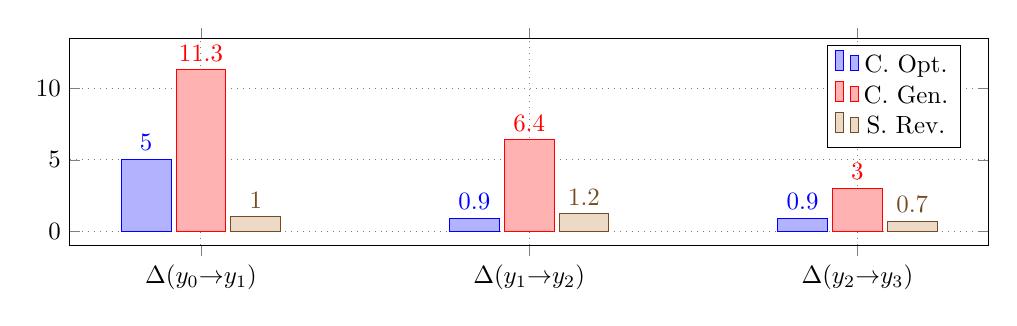
\begin{tikzpicture}[scale=0.9]
\centering
\begin{axis}[
    ybar,
    enlarge x limits=0.2,
    symbolic x coords={$\Delta$($y_0$$\rightarrow$$y_1$), $\Delta$($y_1$$\rightarrow$$y_2$), $\Delta$($y_2$$\rightarrow$$y_3$)},
    xtick=data,
    x tick label style={rotate=0},
    legend pos=north east,
    bar width=20pt,
    nodes near coords,
    height=4.5cm,
    width=1.2\textwidth,
    ymin=-1, ymax=13.5,
    ymajorgrids=true,
    grid = major,
    major grid style={dotted,gray},
]
\addplot coordinates {($\Delta$($y_0$$\rightarrow$$y_1$), 5.0) ($\Delta$($y_1$$\rightarrow$$y_2$), 0.9) ($\Delta$($y_2$$\rightarrow$$y_3$), 0.9)};
\addplot coordinates {($\Delta$($y_0$$\rightarrow$$y_1$), 11.3) ($\Delta$($y_1$$\rightarrow$$y_2$), 6.4) ($\Delta$($y_2$$\rightarrow$$y_3$), 3.0)};
\addplot coordinates {($\Delta$($y_0$$\rightarrow$$y_1$), 1.0) ($\Delta$($y_1$$\rightarrow$$y_2$), 1.2) ($\Delta$($y_2$$\rightarrow$$y_3$), 0.7)};
\legend{C. Opt., C. Gen., S. Rev.}
\draw [->] (axis description cs:1.05,-0.1) -- (axis description cs:0.95,-0.1);
\end{axis}
\end{tikzpicture}
\end{minipage}

\caption{\textbf{Left}: Iteration-wise score improvements. Early iterations significantly improve output quality, and scores generally keep improving with more iterations. \textbf{Right}: \ours Performance improvements with iterations. Most gains($\Delta$) are in the initial iterations for both Code Opt. and \sentxfer.
The numbers are averaged over \chatgpt, \gptt, and \gptf. Task abbreviations: C. Opt. (Code Optimiz.), S. Rev. (Sentiment Reversal), C. Gen. (Constrained Generation).}
\label{fig:iter_score_improvements}
\end{figure}

\paragraph{How important are the multiple iterations of \fbmod-\itermod?}
\Cref{fig:iter_score_improvements} demonstrates that 
on average, the quality of the output improves as the number of iterations increases. 
For instance, in the Code Optimization task, the initial output ($y_0$) has a score of 22.0, which improves to 28.8 after three iterations ($y_3$). Similarly, in the Sentiment Reversal task, the initial output has a score of 33.9, which increases to 36.8 after three iterations. This trend of improvement is also evident in Constrained Generation, where the score increases from 29.0 to 49.7 after three iterations.
\Cref{fig:iter_score_improvements} highlights the diminishing returns in the improvement as the number of iterations increases. Overall, having multiple \fbmod-\itermod iterations significantly enhances the quality of the output, although the marginal improvement naturally decreases with more iterations. 

\begin{figure}[t!]
\begin{subfigure}[t]{.5\textwidth}
\centering
\begin{minipage}[c][8cm]{\linewidth}
\setminted{bgcolor=Box1Color}
\begin{minted}[fontsize=\footnotesize, frame=single, breaklines]{python}
# Slower code
def solve(amount):
  best_price = (amount + 199) // 200 * 380
  # First loop
  for a in range(amount // 200 + 1):
    # ... 4 nested loops ...
    for c1 in range(amount // 1500 + 1):
      if a*200 + b*300 == amount:
        price = a*380 + b*550
        if price < best_price:
          best_price = price
  return best_price
\end{minted}
\end{minipage}
\end{subfigure}%
\begin{subfigure}[t]{.5\textwidth}
\centering
\begin{minipage}[c][8cm]{\linewidth}
\setminted{bgcolor=Box3Color}
\begin{minted}[fontsize=\footnotesize, frame=single, breaklines]{python}
# Faster code
def solve(amount):
  coins = [200, 300]
  prices = [380, 550]
  dp = [float('inf')] * (amount + 1)
  dp[0] = 0
  for i in range(len(coins)):
    for j in range(coins[i], amount+1):
      dp[j] = min(dp[j], dp[j - coins[i]] + prices[i])
  return dp[amount]
\end{minted}

\end{minipage}
\end{subfigure}
\caption{Comparison of code generated by~\citet{pie} (left) and the output after applying \ours (right). The initial code by the baseline, which is nearly identical to the slower input program, fails to improve the efficiency and merely alters the logic for reading input. \ours first generates feedback that diagnoses 
\sethlcolor{Box2Color}
that \hl{\textit{This code is slow because it is using six nested loops to iterate through all possible combinations of coins to pay the amount}}, and suggests that \hl{\textit{a more efficient approach would be ...}}.
\ours then uses this feedback to generate the revised code (right), reducing the time complexity to $\mathcal{O}(amount*coins)$. 
The full example is provided in \Cref{sec:additionalanalysis}
}
\label{fig:analysis_example}
\end{figure}

The performance may not always monotonically increase with iterations: in multi-aspect feedback tasks like \acrogen, where the output quality can vary during iteration with improvement in one aspect but decline in another aspect. To counter this, \ours generates numerical scores for different quality aspects, leading to a balanced evaluation and appropriate output selection. 


\paragraph{Can we just generate multiple outputs instead of refining?}

Does \ours improve because of the iterative refinement, or just because it generates \emph{more} outputs? 
We compare \ours with \chatgpt, when \chatgpt generates $k=4$ samples (but without feedback and refinement). 
Then, we compare the performance of \ours against these $k$ initial outputs in a 1 vs. $k$ evaluation. In other words, we assess whether \ours can outperform \emph{all} $k$ initial outputs.
The results of this experiment are illustrated in Figure \ref{fig:refinement-vs-sampling-analysis} (\Cref{sec:additionalanalysis}).  Despite the increased difficulty of the 1 vs. $k$ setting,  the outputs of \ours are still preferred by humans over \emph{all} $k$ initial outputs.
This shows the importance of refinement according to feedback over the alternative of just generating multiple initial outputs.




\paragraph{Does \ours work with weaker models?}
The experiments in \Cref{sec:results} were performed with some of the strongest available models; does \ours work with smaller or weaker models as well?
To investigate this, we instantiated \ours with Vicuna-13B \citep{chiang2023vicuna}, a less powerful base model. While Vicuna-13B is capable of generating initial outputs, it struggles significantly with the refinement process.
Specifically, Vicuna-13B was not able to consistently generate the feedback in the required format. Furthermore, even when provided with Oracle or hard-coded feedback, it often failed to adhere to the prompts for refinement. Instead of refining its output, Vicuna-13B either repeated the same output or generated a hallucinated conversation, rendering the outputs less effective. We thus hypothesize that since Vicuna-13B was trained on conversations, it does not generalize as well as instruction-based models to test-time few-shot tasks. 
Example output and analysis is provided in \Cref{sec:vicunaresults}.



\paragraph{Qualitative Analysis}

We conduct a qualitative analysis of the feedback generated by \ours and its subsequent refinements. We manually analyze 70 samples in total (35 success cases and 35 failure cases) for \codeopt~\citep{pie} and \gsm~\citep{cobbe2021training}. For both \gsm and \codeopt, we found that the feedback was predominantly actionable, with the majority identifying problematic aspects of the original generation and suggesting ways to rectify them.















When \ours failed to improve the original generation, the majority of issues were due to erroneous feedback rather than faulty refinements. Specifically, 33\% of unsuccessful cases were due to feedback inaccurately pinpointing the error's location, while 61\% were a result of feedback suggesting an inappropriate fix. Only 6\% of failures were due to the refiner incorrectly implementing good feedback. These observations highlight the vital role of accurate feedback plays in \ours.

In successful cases, the refiner was guided by accurate and useful feedback to make precise fixes to the original generation in 61\% of the cases. Interestingly, the refiner was capable of rectifying issues even when the feedback was partially incorrect, which was the situation in 33\% of successful cases. This suggests resilience to sub-optimal feedback. Future research could focus on examining the refiner's robustness to various types of feedback errors and exploring ways to enhance this resilience. 
In Figure \ref{fig:analysis_example}, we illustrate how \ours significantly improves program efficiency by transforming a brute force approach into a dynamic programming solution, as a result of insightful feedback. Additional analysis on other datasets such as \dialgen is provided in \Cref{sec:additionalanalysis}.




\paragraph{Going Beyond Benchmarks}
While our evaluation focuses on benchmark tasks, \ours is designed with broader applicability in mind. We explore this in a real-world use case of website generation, where the user provides a high-level goal and \ours assists in iteratively developing the website. Starting from a rudimentary initial design, \ours refines HTML, CSS, and JS to evolve the website in terms of both usability and aesthetics. This demonstrates the potential of \ours in real-world, complex, and creative tasks. See \Cref{sec:beyondbenchmarks} for examples and further discussion, including broader, societal impact of our work.









